\section{Ejercicios de Ajax en w3schools}

Capturas de pantalla:

\begin{figure}[H]
    \centering
    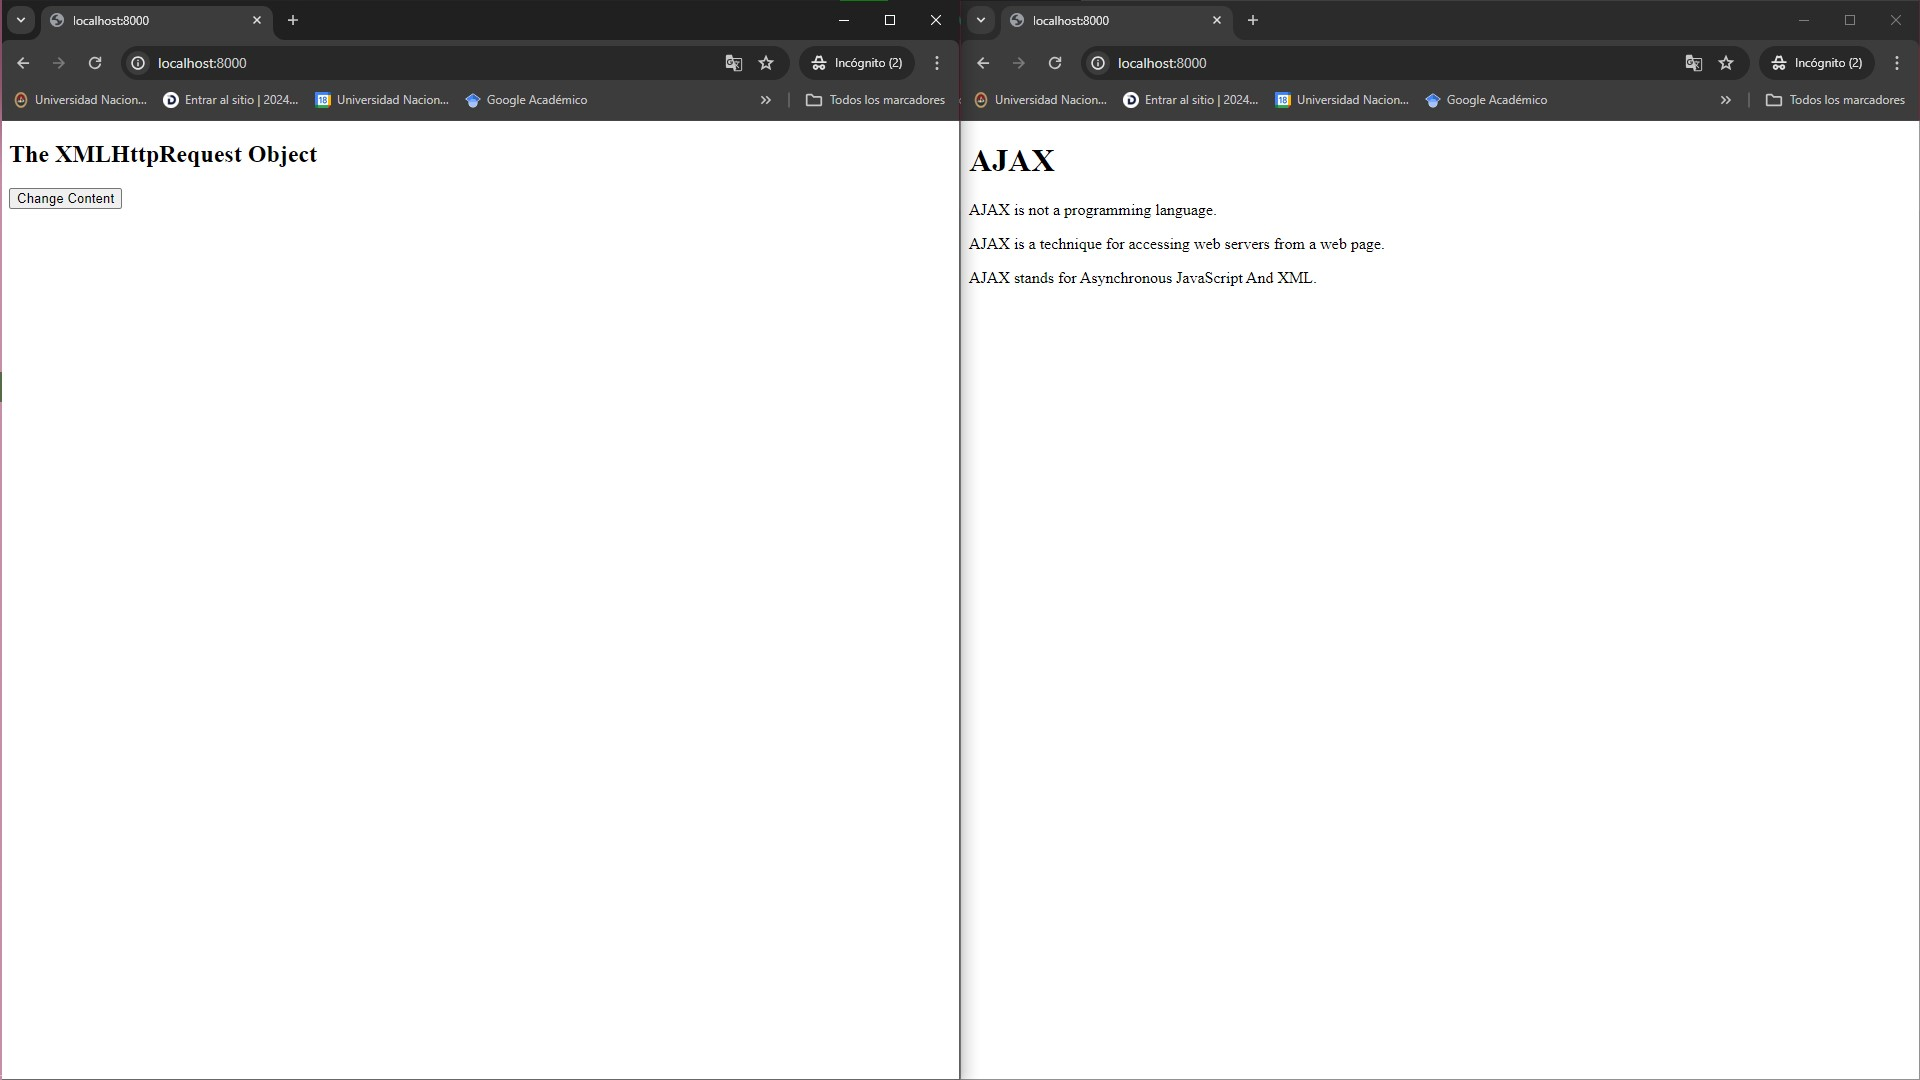
\includegraphics[width=0.7\textwidth]{img/ex1.jpg}
    \caption{Creando un objeto XMLHttpRequest}
    \end{figure}


\begin{figure}[H]
  \centering
  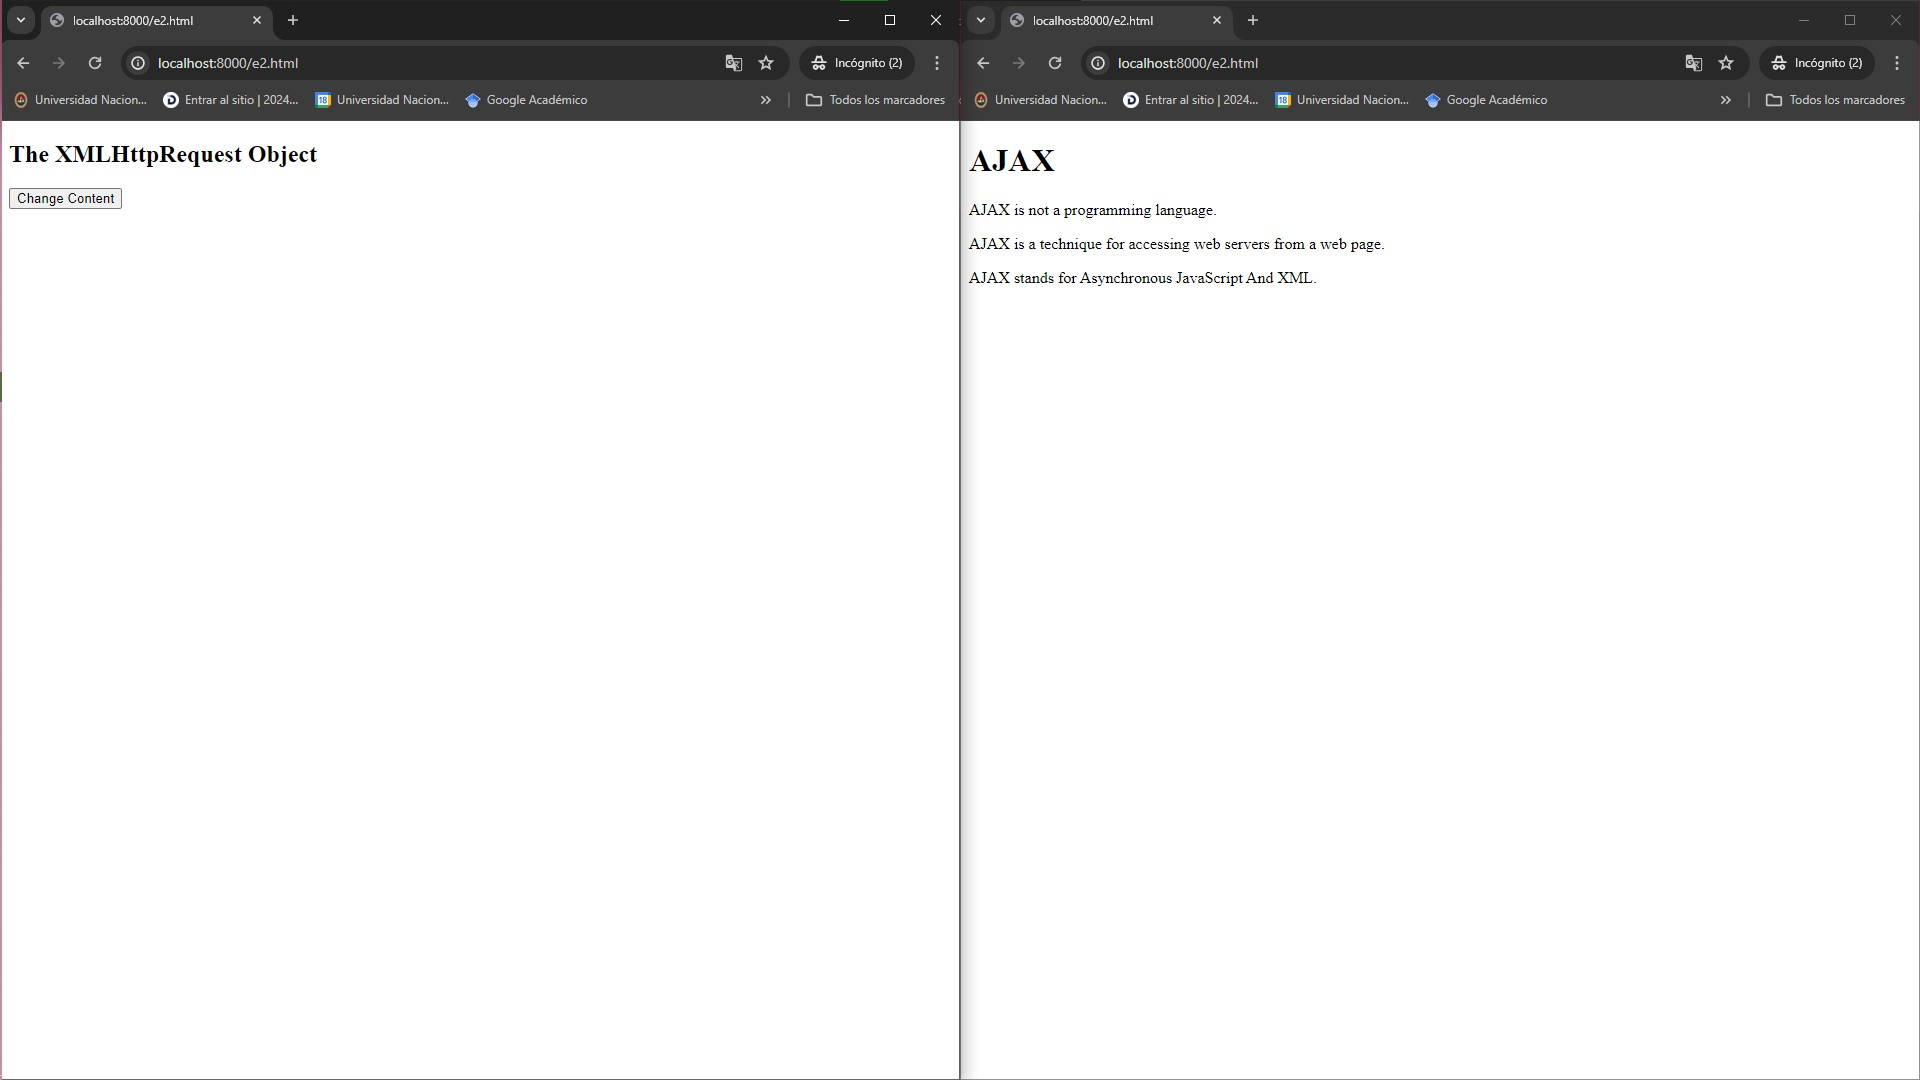
\includegraphics[width=0.7\textwidth]{img/ex2.jpg}
  \caption{Creando otro objeto XMLHttpRequest}
  \end{figure}
\begin{figure}[H]
    \centering
    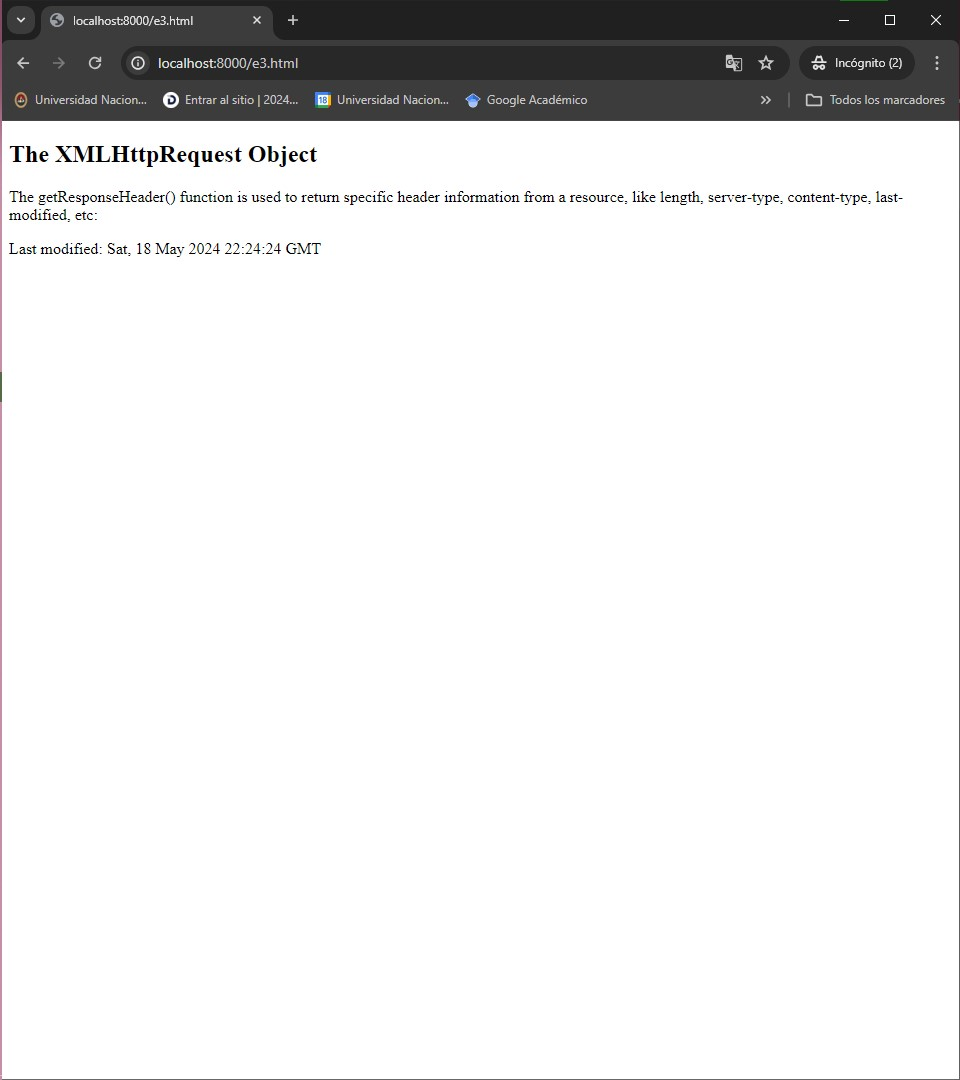
\includegraphics[width=0.5\textwidth]{img/ex3.jpg}
    \caption{Modificando el objeto XMLHttpRequest}
    \end{figure}
\begin{figure}[H]
    \centering
    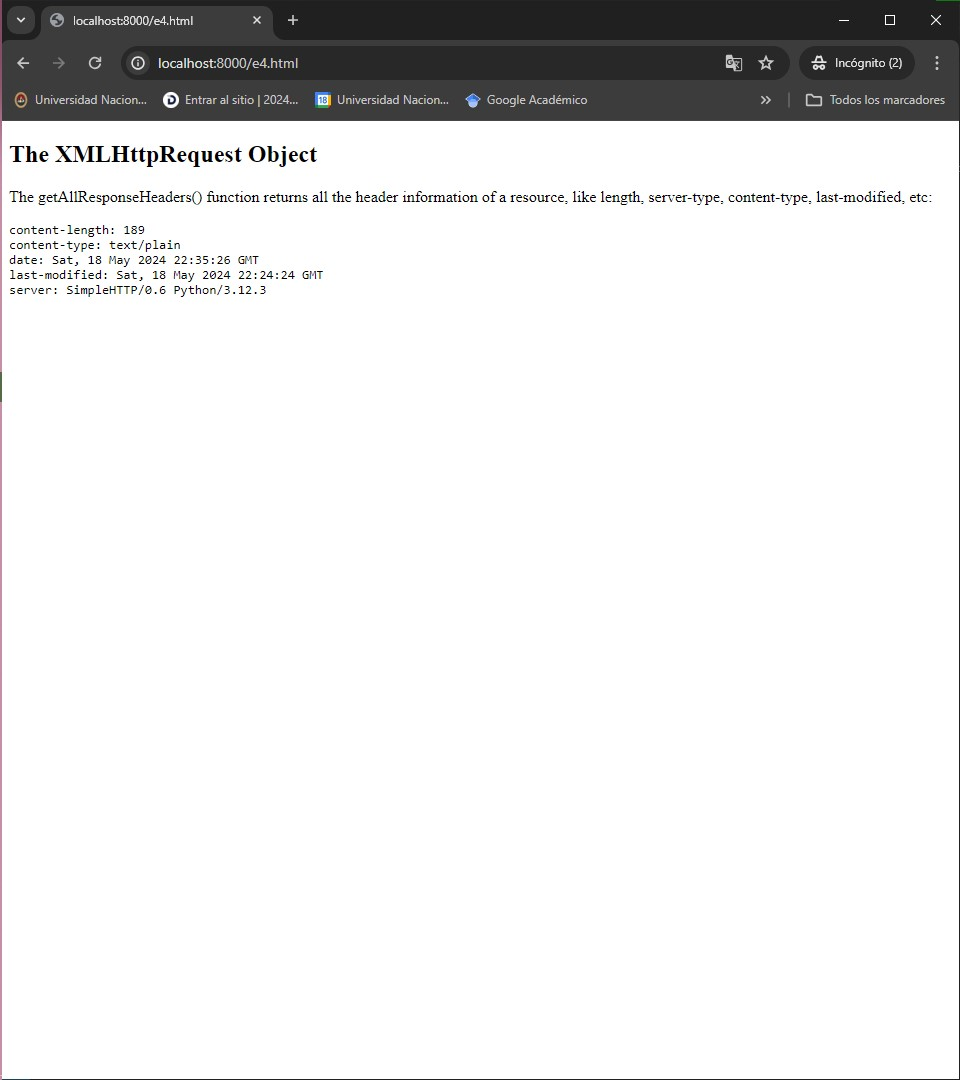
\includegraphics[width=0.5\textwidth]{img/ex4.jpg}
    \caption{Añadiendo contenido al objeto XMLHttpRequest}
    \end{figure}

\begin{figure}[H]
      \centering
      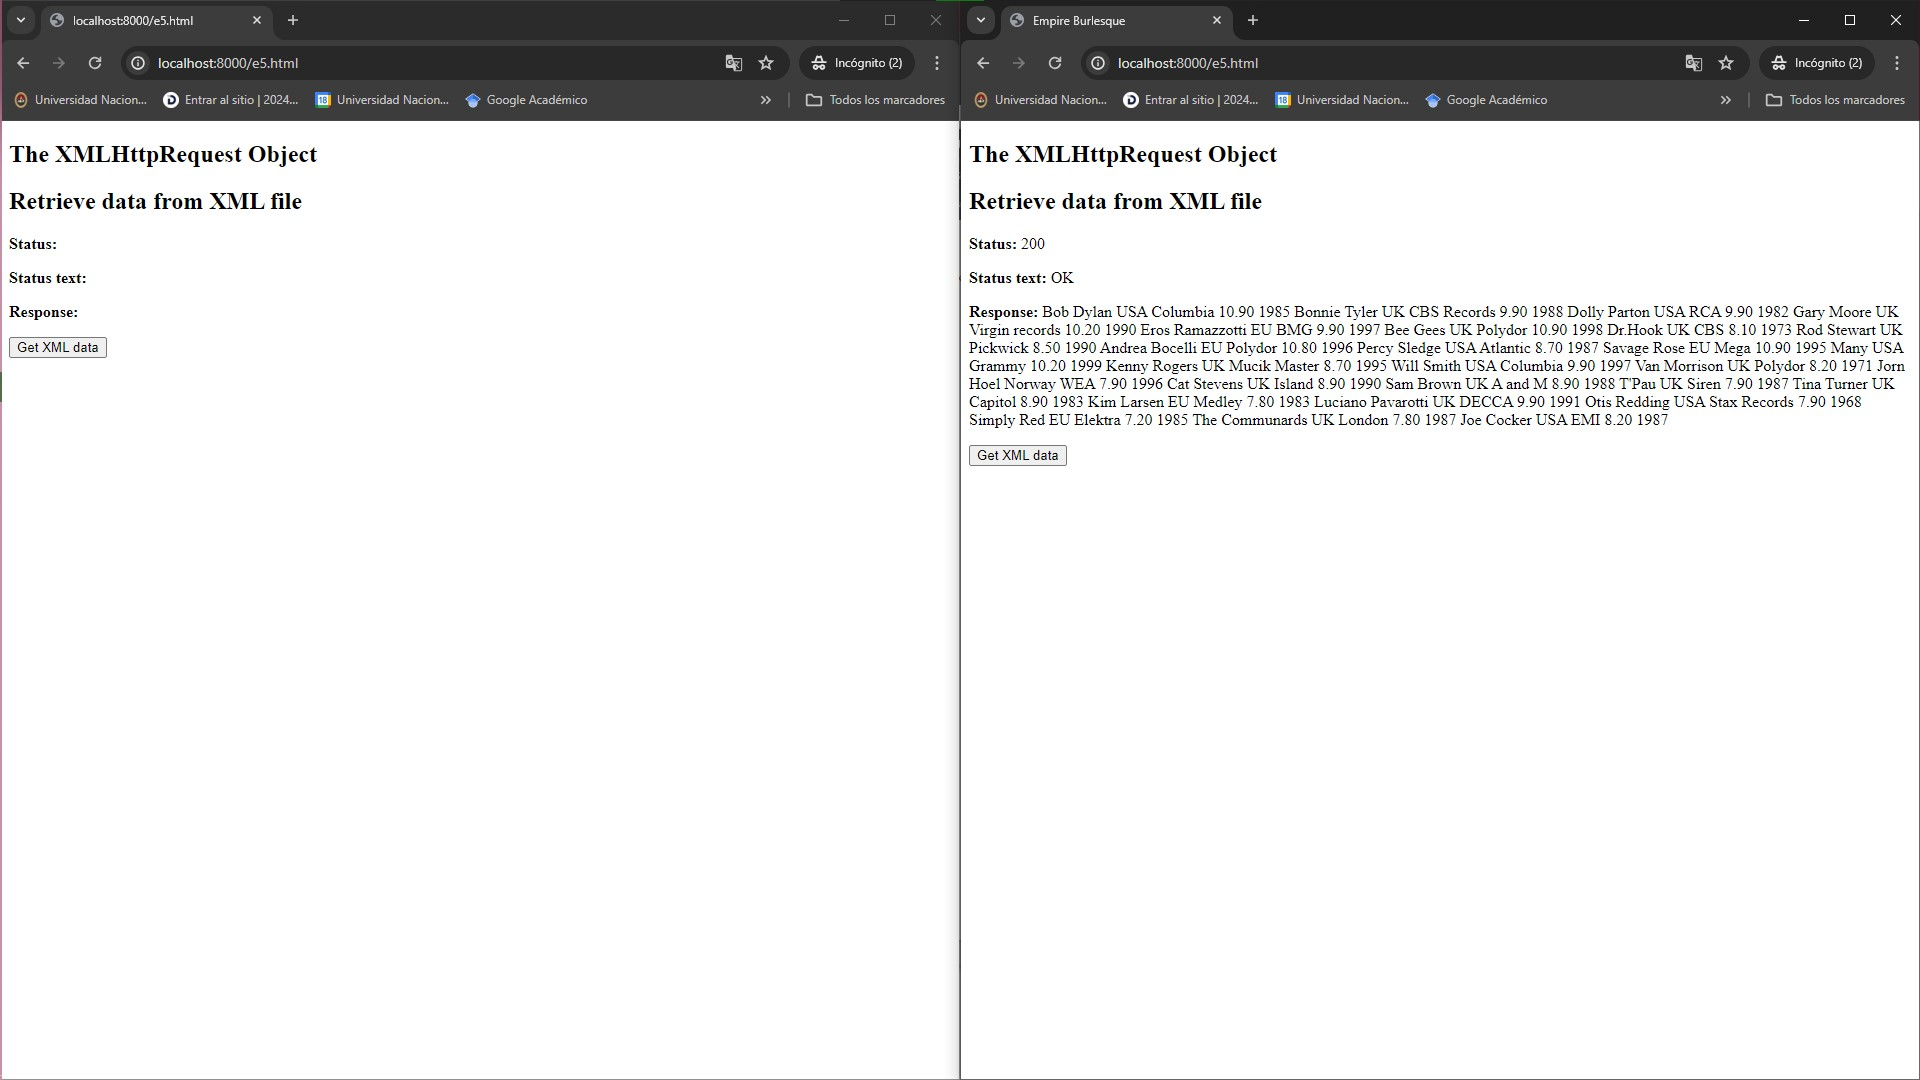
\includegraphics[width=0.7\textwidth]{img/ex5.jpg}
      \caption{Pidiendo un reporte del status del objeto XMLHttpRequest}
      \end{figure}

\begin{figure}[H]
    \centering
    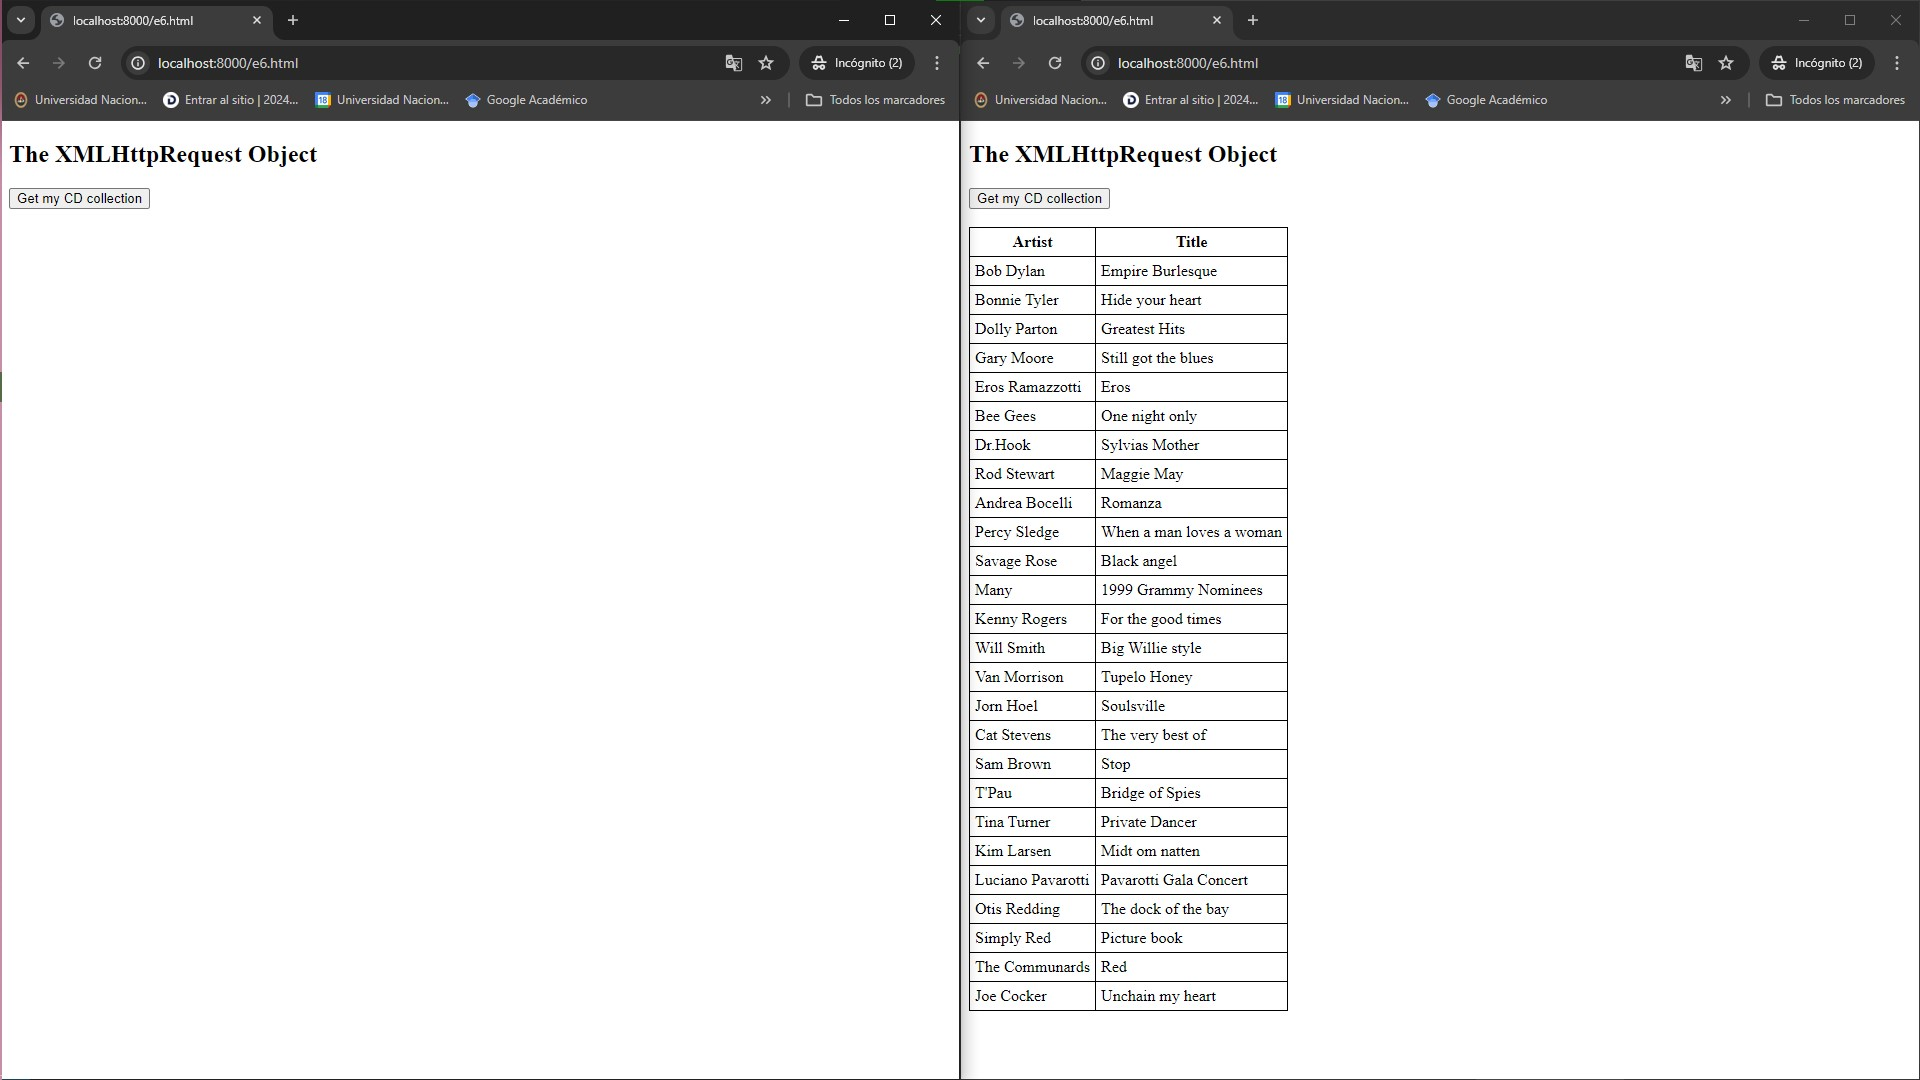
\includegraphics[width=0.7\textwidth]{img/ex6.jpg}
    \caption{Obtener informacion a travez de Ajax de un archivo XML}
    \end{figure}

\begin{figure}[H]
  \centering
  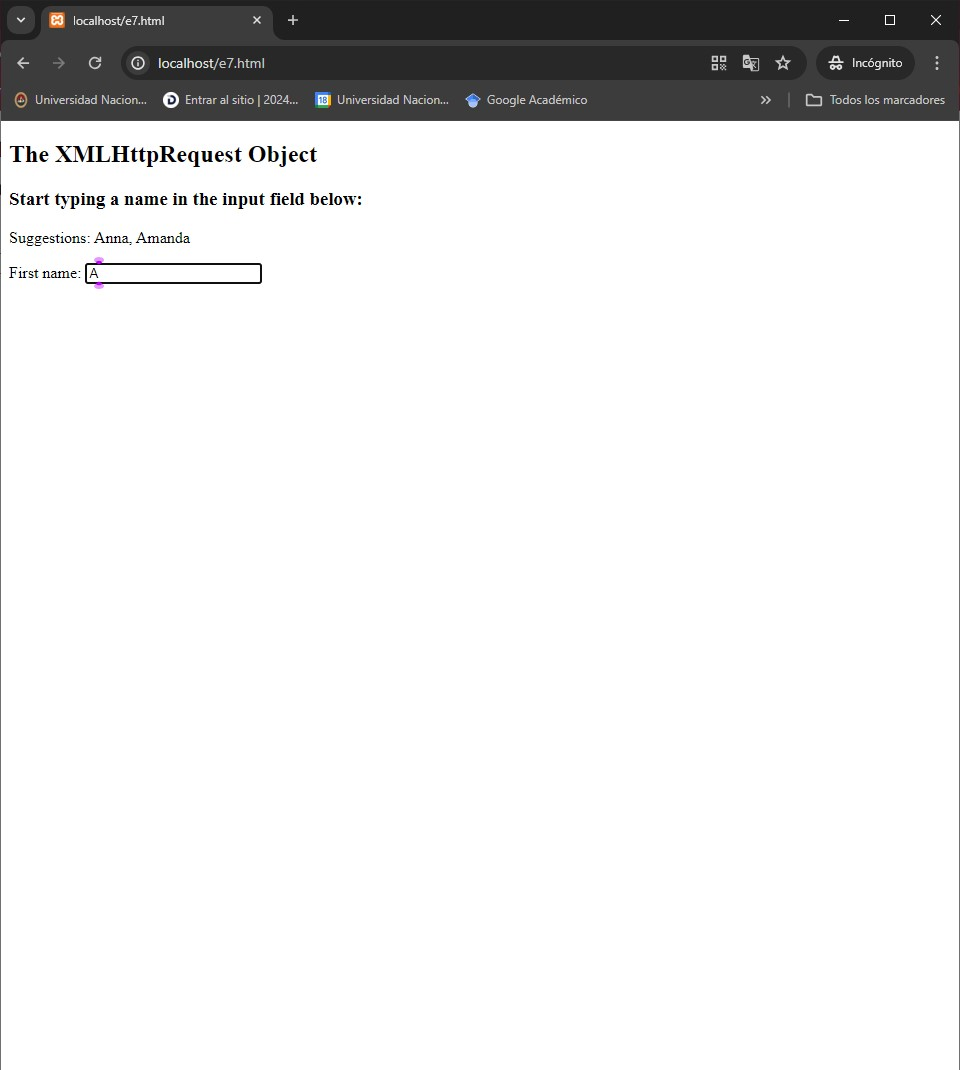
\includegraphics[width=0.5\textwidth]{img/ex7.jpg}
  \caption{Comunicacion entre un servidor web y una pagina web mientras se ingresan datos}
  \end{figure}

\begin{figure}[H]
  \centering
  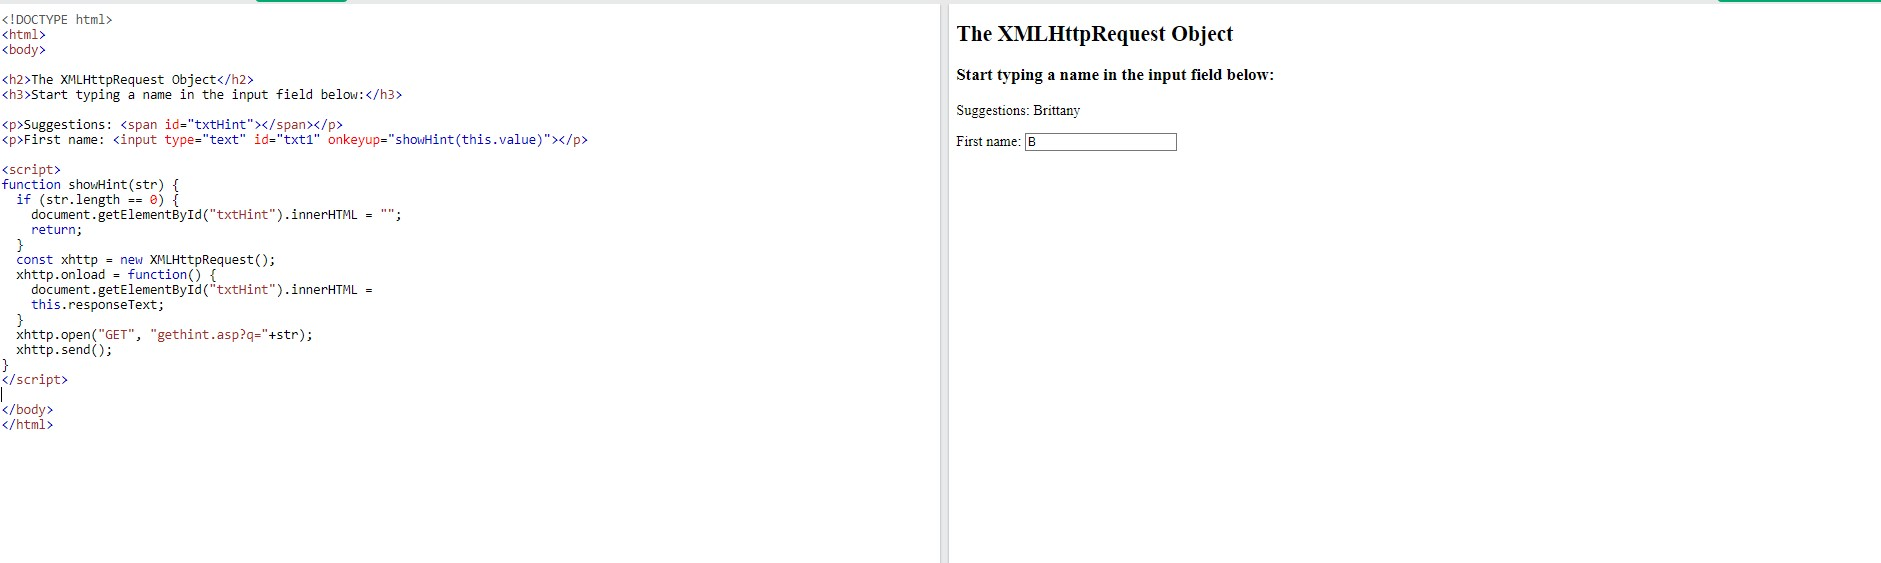
\includegraphics[width=0.7\textwidth]{img/ex8.jpg}
  \caption{Obtener informacion de una base de datos usando Ajax}
  \end{figure}

\begin{figure}[H]
  \centering
  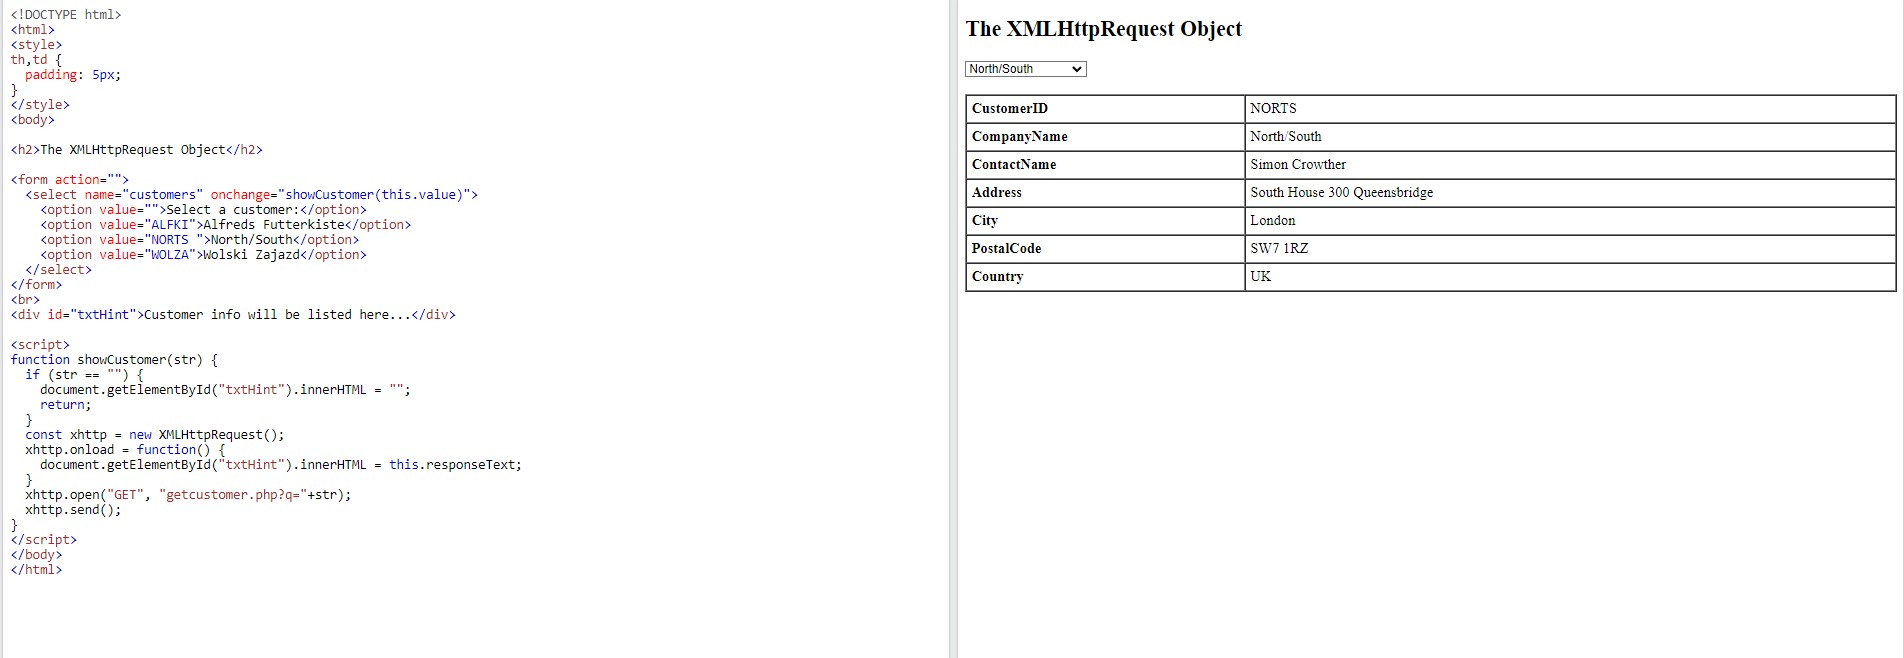
\includegraphics[width=0.7\textwidth]{img/ex9.jpg}
  \caption{Mostrando datos en una tabal HTML}
  \end{figure}

\begin{figure}[H]
    \centering
    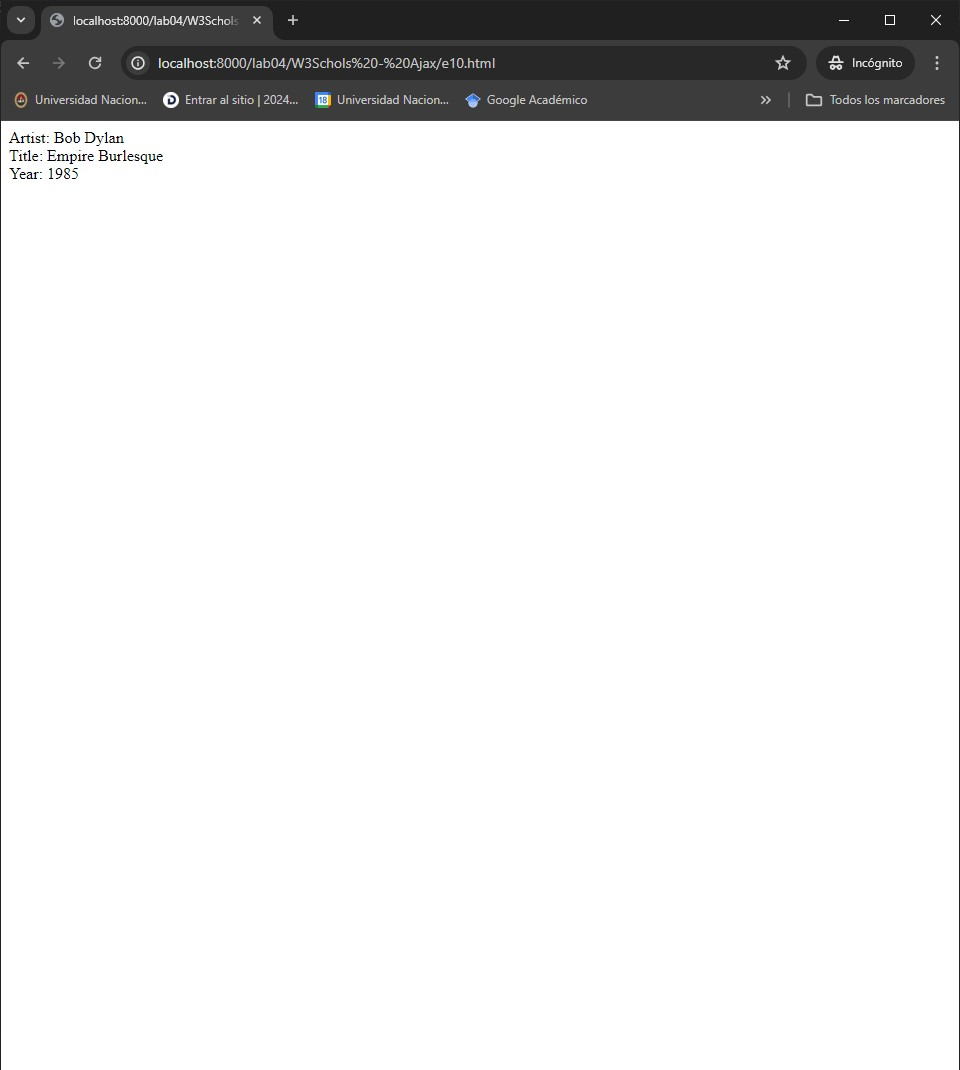
\includegraphics[width=0.5\textwidth]{img/ex10.jpg}
    \caption{ Pidiendo informacion de la base de datos}
    \end{figure}

\begin{figure}[H]
  \centering
  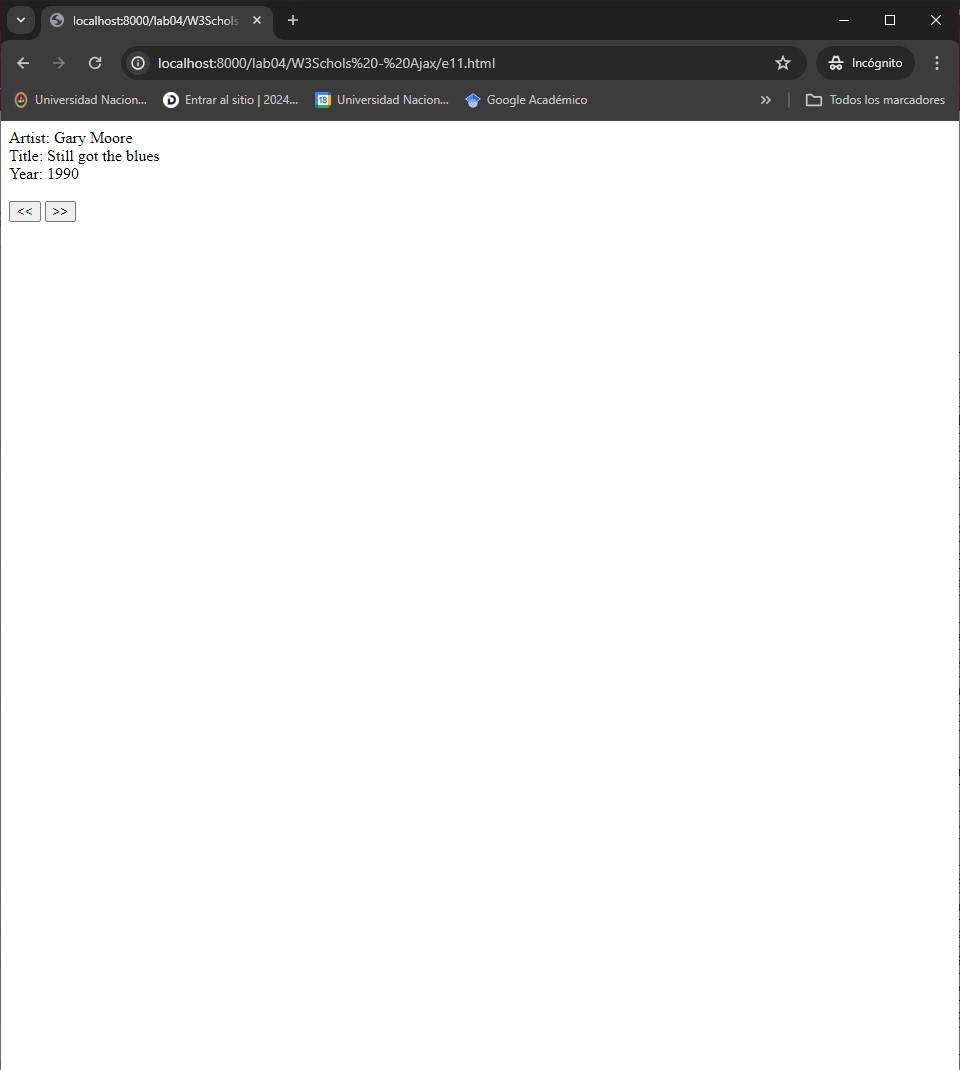
\includegraphics[width=0.5\textwidth]{img/ex11.jpg}
  \caption{Recorriendo la informacion de la base de datos}
  \end{figure}

\begin{figure}[H]
  \centering
  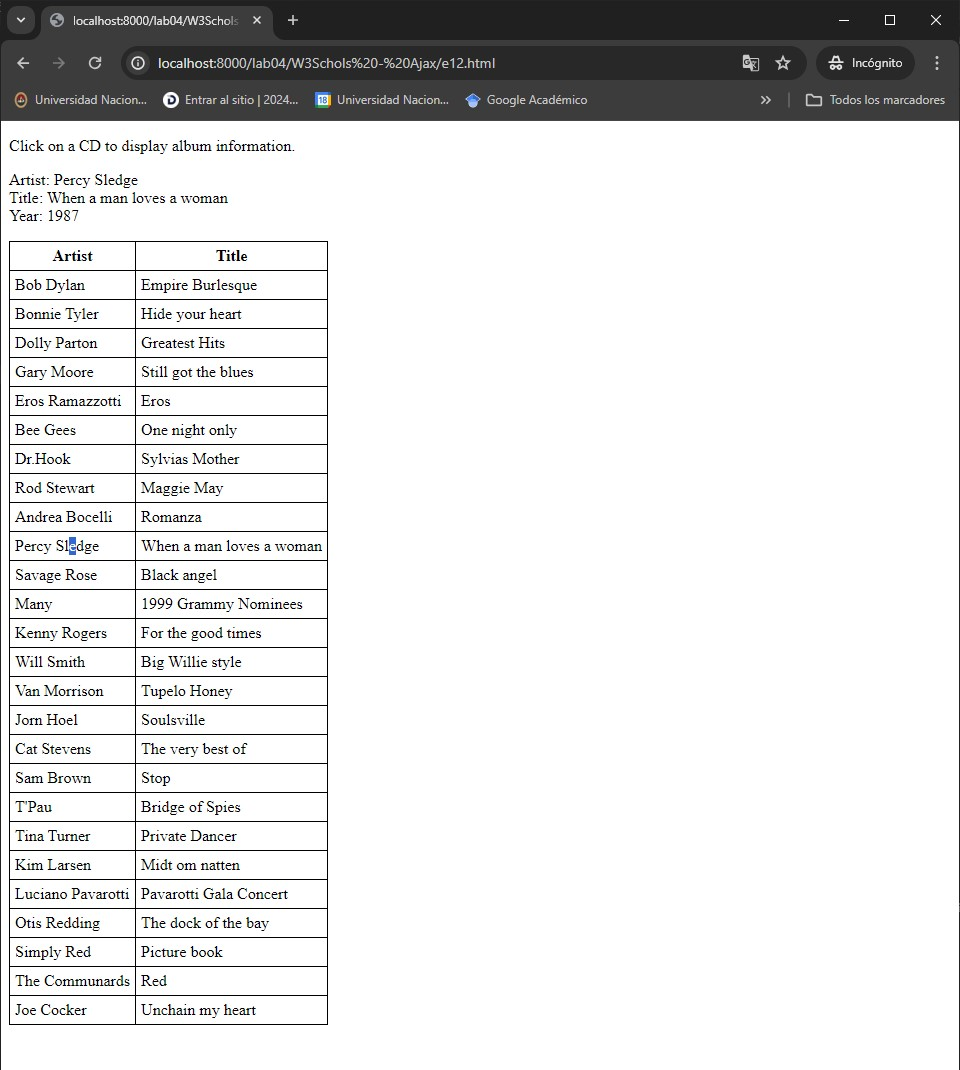
\includegraphics[width=0.5\textwidth]{img/ex12.jpg}
  \caption{Mostrar los elementos en una tabla HTML}
  \end{figure}